\documentclass[tikz,border=5pt]{standalone}
\usepackage{tikz}
\usetikzlibrary{decorations.pathmorphing}

\begin{document}

% Wavefunction matching illustration
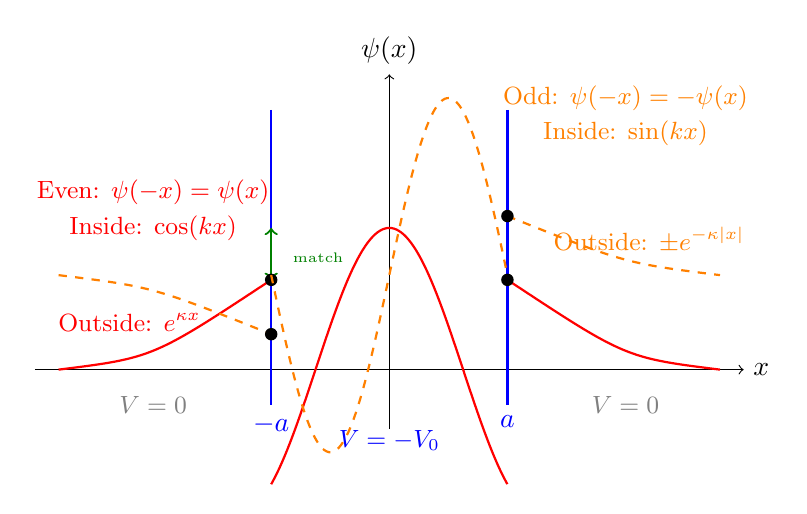
\begin{tikzpicture}[scale=1.5]

% Axes
\draw[->] (-3,0) -- (3,0) node[right] {$x$};
\draw[->] (0,-0.5) -- (0,2.5) node[above] {$\psi(x)$};

% Potential well boundaries
\draw[thick,blue] (-1,2.2) -- (-1,-0.3) node[below] {$-a$};
\draw[thick,blue] (1,2.2) -- (1,-0.3) node[below] {$a$};
\node[blue,font=\small] at (0,-0.6) {$V = -V_0$};
\node[gray,font=\small] at (-2,-0.3) {$V = 0$};
\node[gray,font=\small] at (2,-0.3) {$V = 0$};

% Even parity wavefunction
\draw[thick,red] (-2.8,0) .. controls (-2,0.1) .. (-1,0.76);
\draw[thick,red,samples=50,domain=-1:1,smooth] plot (\x, {1.2*cos(deg(0.8*pi*\x))});
\draw[thick,red] (1,0.76) .. controls (2,0.1) .. (2.8,0);

% Label for even parity
\node[red,font=\small] at (-2,1.5) {Even: $\psi(-x) = \psi(x)$};
\node[red,font=\small] at (-2,1.2) {Inside: $\cos(kx)$};
\node[red,font=\small] at (-2.2,0.4) {Outside: $e^{\kappa x}$};

% Matching point annotation
\draw[green!50!black,thick,<->] (-1,1.2) -- (-1,0.76);
\node[green!50!black,font=\tiny,right] at (-0.9,0.95) {match};

% Continuity markers
\fill[black] (-1,0.76) circle (1.5pt);
\fill[black] (1,0.76) circle (1.5pt);

% Odd parity wavefunction (shifted up for clarity)
\begin{scope}[yshift=0.8cm]
\draw[thick,orange,dashed] (-2.8,0) .. controls (-2,-0.1) .. (-1,-0.5);
\draw[thick,orange,dashed,samples=50,domain=-1:1,smooth] plot (\x, {1.5*sin(deg(pi*\x))});
\draw[thick,orange,dashed] (1,0.5) .. controls (2,0.1) .. (2.8,0);

\node[orange,font=\small] at (2,1.5) {Odd: $\psi(-x) = -\psi(x)$};
\node[orange,font=\small] at (2,1.2) {Inside: $\sin(kx)$};
\node[orange,font=\small] at (2.2,0.3) {Outside: $\pm e^{-\kappa|x|}$};

\fill[black] (-1,-0.5) circle (1.5pt);
\fill[black] (1,0.5) circle (1.5pt);
\end{scope}

\end{tikzpicture}

\end{document}
